\newpage
\chapter{Empirical Risk Minimization and PAC Learning}

In this chapter, we will introduce the concept of \textbf{Empirical Risk Minimization} (ERM) in which to frame learning problems, the notion of inductive bias, and the main results of algorithmic learnability, encapsulated in the definition of \textbf{Probably Approximately Correct} (PAC) Learning and of complexity of a set of hypothesis, namely
VC-dimension and Rademacher complexity.

\section{Empirical Risk Minimization}

We begin by considering a supervised learning setting in which the \textbf{input space} $X$ is a subset of $\mathbb{R}^n$, and the \textbf{output space} $Y$ can be real-valued (e.g., $Y = \mathbb{R}$), binary (e.g., $Y = \{0,1\}$), or a finite set of classes (e.g., $Y = \{0,1,\ldots,K\}$). In this probabilistic framework, each input-output pair $(x,y)$ is drawn from a joint probability distribution
$$
p(x,y) \;\in\; \mathrm{Dist}(X \times Y),
$$
often referred to as the \emph{\textbf{data generating distribution}}. 

By definition, this distribution factors into the marginal $p(x)$ and the conditional $p(y \mid x)$, so that
$$
p(x,y) \;=\; p(x)\,p(y \mid x).
$$

Because $p(x)$ and $p(y \mid x)$ describe how inputs and outputs are related, it is helpful to write them explicitly. The marginal distribution of $x$ is
$$
p(x) \;=\; \int p(x,y)\,dy,
$$
while the conditional distribution of $y$ given $x$ is
$$
p(y \mid x) \;=\; \frac{p(x,y)}{p(x)}.
$$

A typical dataset $D$ in supervised learning consists of $N$ input-output pairs drawn independently from $p(x,y)$. We denote this as
$$
D \sim p^N(x,y),
$$
which means
$$
D \;=\; \{(x_i, y_i) \,\mid\, i = 1, \dots, N\},
$$
where each $(x_i, y_i)$ is sampled according to the joint distribution $p(x,y)$. 

In many cases, we assume that $p(y \mid x)$ depends on some unknown function of $x$. Formally, one might write
$$
p(y \mid x) \;=\; p\bigl(y \mid f(x)\bigr),
$$
where $f$ is the function we aim to learn. The central objective in supervised learning—through methods such as empirical risk minimization—is to find or approximate this function $f$ by using the observed data $D$.

\section{Risk and Empirical Risk}

$h \in \mathcal{H} \quad x,y \sim p(x,y)$

\textbf{\textit{loss function}} $l(x,y,h) \in \mathbb{R_{\ge 0}}$, 

\begin{itemize}
    \item 0-1 loss: $l(x,y,h) = \mathbb{I}(h(x) \neq y)$, eith $y \in \{0, 1\}$.
    \item squared loss: $l(x,y,h) = (h(x) - y)^2$, with $y \in \mathbb{R}$.
\end{itemize}

We have a probabilistic process, so we have some inputs that are more likely than others. If a model makes a mistake on a more likely input, it should be penalized more.

\begin{definitionblock}[Risk]
The \textbf{\textit{risk}} (or \textbf{\textit{generalization error}}) is defined as:
$$
R(h) = E_{x,y \sim p(x,y)}[l(x,y,h)]
$$ 
\end{definitionblock}

\textbf{Risk minimization principle:}

The goal is to find the hypothesis $h$ that minimizes the risk.
$$
\text{find } h^* \in \mathcal{H} \text{ such that } h^* = \mathrm{arg\,min}_{h \in \mathcal{H}} R(h)
$$

\begin{definitionblock}[Empirical Risk]
The \textbf{\textit{empirical risk}} (or \textbf{\textit{training error}}) is defined as:
$$
\hat R = \dfrac 1N \sum_{i=1}^N l(x_i, y_i, h)
$$
\end{definitionblock}


\textbf{Empirical risk minimization principle:}

The goal is to find the hypothesis $h$ that minimizes the empirical risk.
$$
\text{find } h^*_D = \mathrm{arg\,min}_{h \in \mathcal{H}} \hat R(h)
$$

\subsection{Bias Variance Trade-off}

In this section, we want to analyze the generalization error and decom-
pose it according to the sources of error that we are going to commit.

In what follows, we will use the squared loss (hence we will focus on
regression problems). Considering $h \in \mathcal H$, an explicit expression of the generalization error committed when choosing hypothesis $h$ is:
$$
R(h) = E_p[l(x,y,h)] = \int \int (h(x) - y)^2 p(x,y) dx dy
$$

\newtheorem{theorem}{Theorem}
\begin{theorem}
    The minimizer of the generalization error $R$ is:
    $$
    \boxed{ g(x) = E[y|x] = \int y p(y|x) dy }
    $$
    so that $g = \mathrm{arg\,min}_h R(h),\ if\ g \in \mathcal H$
\end{theorem}

We can rewrite the risk as:
$$
R(h) = \underbrace{\int (h(x) - g(x))^2 p(x) dx}_{=\ 0 \quad iff \quad h(x) = g(x)} + \overbrace{\iint (g(x) - y)^2 p(x,y) dx dy}^{\text{independent of }h \text{: intrinsic noise}}
$$



$$
\begin{array}{rl}
E_D[R(h^*_D)]
& = \underbrace{\int ( E_D[h^*_D(x) - g(x)])^2 p(x) dx}_{bias^2} \\
& + \underbrace{\int E_D[(h^*_D(x) - E_D[h^*_D(x)])^2 p(x) dx]}_{variance} \\
& + \underbrace{\iint (g(x) - y)^2 p(x,y) dx dy}_{noise}
\end{array}
$$

\section{ERM and Maximum Likelihood}

Given a dataset $D = \{(x_i, y_i)\}_{i=1, \dots, m}$ s.t. $D \sim p^m, p = p(x,y)$

We factorize the data generating distributions as: $p(x,y) = p(x) p(y|x)$ and we make an hypothesis on $p(y|x)$, trying to express this conditional probability in a parametric form:
$$p(y|x) = p(y|x, \theta)$$

[check recording for missing part]

We consider the log Likelihood:
$$
L(\theta; D) = \sum_{i = 1}^m \log p(y_i | x_i, \theta)
$$

Then we apply the maximum likelihood principle:

$$
\begin{array}{rcl}
    \argmin{\theta} - L(\theta; D) &
    = & \argmin{\theta} - \dfrac 1m \displaystyle\sum_{i=1}^m \log p(y_i | x_i, \theta) \\
    & = & \argmin{\theta}\ E_{p(x,y)}[-\log p(y | x, \theta)]
\end{array}
$$

since the avarage is an empirical approximation of the expectation.

\begin{observationblock}[Empirical Risk]
$$
-\frac{1}{m}\sum_{i=1}^{m}\log p(y_i|x_i, \theta) \text{is known as \textbf{empirical risk}}
$$
\end{observationblock}



\section{KL divergence}

Consider a probability distribution $p(x)$, then $-\log p(x)$ is a measure of \textbf{self-information}. Indeed, if $p(x) = 1$ then $-\log p(x) = 0$ (no self-information), describing substantially out (lack of) surprise in observing the event. If instead $p(x) = 0$ then $-\log p(x) = \infty$. In general, the more rare the event is, i.e. the lower is $p(x)$, the more self-information it carries, i.e. the larger is $-\log p(x)$.

\begin{definitionblock}[Entropy]
    In an information-theoretic sense, the \textbf{entropy} is a measure of the inforamtion that is carries by a random phenomenon, expressed as the expected amount of self-information that is conveyed by a realization of the random phenomenon.
    
    It is formally defined as:
    $$
    H(p) = E_p[-\log p(x)] = -\int p(x) \log p(x) dx
    $$
    for the continuous case, and:
    $$
    H(p) = E_p[-\log p(x)] = -\sum p(x) \log p(x)
    $$
    for the discrete case.
\end{definitionblock}

For the discrete case, the maximum entropy is achieved for te uniform distrivution and is equal to $\log n$, where $n$ is the number of possible outcomes. In the continuous case, for a fixed variance, the distribution that maximizes the entropy is the Gaussian. The entropy is always 0 if we have a deterministic distribution.

\begin{definitionblock}[Kullback-Leibler divergence]
    The \textbf{Kullback-Leibler divergence} (or \textbf{relative entropy}) between two probability distributions $p(x)$ and $q(x)$ is a measure of how one distribution diverges from a second, expected probability distribution.
    
    It is formally defined as:
    $$
    D_{KL}(p||q) = E_p\left[\log \dfrac{p(x)}{q(x)}\right] = \int p(x) \log \dfrac{p(x)}{q(x)} dx
    $$
    for the continuous case, and:
    $$
    D_{KL}(p||q) = E_p\left[\log \dfrac{p(x)}{q(x)}\right] = \sum p(x) \log \dfrac{p(x)}{q(x)}
    $$
    for the discrete case.
\end{definitionblock}

Intuitively, we are taking a sort of expected difference between $p$ and $q$, expressed in terms of a log odds ratio. It tells us how different two distributions are: the larger \textit{KL} the more different are $p$ and $q$.

Properties of \textit{KL}:
\begin{itemize}
    \item $KL[q||p]$ is a convex function of $q$ and $p$ and $KL[q||p] \ge 0$
    \item KL is non-symmetric, i.e. $KL[q||p] \neq KL[p||q]$
    \item $KL[q||p] = -H[q] - \mathbb{E}_q[\log p]$, where the first term is the entropy and the second term is known as cross-entropy between $p$ and $q$.
\end{itemize}


Suppose moreover, that $p$ is fixed but unknown, $q = q_0$ can vary: what we usually do is trying to find the best $q_{\theta}$ that approximates $p$.

The \textbf{mutual information} between $x$ and $y$ is defined as:
$$
I(x,y) = KL[p(x,y)||p(x)p(y)] = \int \int p(x,y) \log \dfrac{p(x,y)}{p(x)p(y)} dx dy
$$

$KL[p(x,y)||p(x)p(y)] = 0$ iff $x$ and $y$ are independent.

Moreover, the more dependent they are, the more different is $p(x,y)$ from the product of the marginals, the more information $x$ carries about $y$ and viceversa.

In other words, the higher the mutual information is, the more knowing $y$ will tell us about $x$, the less residual uncertainty on $x$ we will have.
\newpage
Consider a dataset: $\underline{x} : x_1,\dots,x_N$:
\begin{definitionblock}[Empirical distribution]
    The \textbf{empirical distribution} of a dataset $\underline{x}$ is defined as:
    $$
    \hat p(\underline{x}) = \dfrac 1N \sum_{i=1}^N \delta(x - x_i)
    $$
    where $\delta(x)$ is the Dirac delta function.
\end{definitionblock}

It is an approximation of the input data generating function$p(x)$. Practically, the more observations we have, the more the empirical distribution will look like $p(x)$.

Given a distribution $q$, we can compute:
$$
KL[p_{emp}||q] = \mathbb{E}_{p_{emp}}\left[\log \dfrac{p_{emp}(x)}{q(x)}\right] = \dfrac 1N \sum_{i=1}^N \log \dfrac{p(x_i)}{q(x_i)}
$$

If $q = q_0$, this is $-\frac{1}{N}L(\Theta)$ plus a constant. Hence maximizing $L(\Theta)$ is essentially equivalent to minimizing the \textit{KL} between $p_{emp}$ and $q_0$. This means that we can always rephrase maximum likelihood in terms of cross-entropy.


\section{PAC Learning}
Our goal is to measure how much we can learn as a function of the model complexity. This results in the \textbf{PAC} (Probably Approximately Correct) \textbf{learning} framework, which encodes the notion of model complexity and gives also bounds on the error that we commit. 
Here we consider it in the context of (binary) classification, i.e. $y \in {0,1}$, using the 0-1 loss. 

\begin{definitionblock}[PAC Learning]
    A realizable hypothesis set $\mathcal{H}$ is \textbf{\textit{PAC learnable}} iff $\forall \epsilon, \delta \in (0,1), \forall p(x,y), \exists m_{\epsilon, \delta} \in \mathcal{N} s.t. \forall m \geq m_{\epsilon, \delta}, \exists D ~ p^m, |D| = m$ then $p_D(R(h^*_D) \leq \epsilon) \geq 1 - \delta$
\end{definitionblock}

This means that, fixing two parameters $\epsilon, \delta \in (0,1)$, governing our precision, and a data generating distribution $p(x,y)$, we can find a number of samples $m_{\epsilon, \delta}$ such that, with probability at least $1 - \delta$, the empirical risk of the best hypothesis $h^*_D$ is less than $\epsilon$. Note that the probability here is over the dataset D, meaning that our learning will succeed for a fraction $1 - \delta$ of sampled datasets. 

In a more general setting, 
\begin{definitionblock}
Given an hypothesis set $\mathcal{H}$ (not necessarily realizable) and an algorithm A, 
$\mathcal{H} is \text{\textbf{agnostic PAC-learnable}} iff \forall \epsilon, \delta \in (0,1), 
\forall p(x,y), \exists m_{\epsilon, \delta} \in \mathcal{N} ~ p^m, 
|D|  = m \geq m_{\epsilon, \delta} \Rightarrow p_D(R(h^*_D) \leq R(h^*) + \epsilon) \geq 1 - \delta$, 
being $h^A_D$ the result of applying A to $\mathcal{H}$ and D.
\end{definitionblock}

This means that, fixing two parameters $\epsilon, \delta \in (0,1)$, governing our precision, and a data generating distribution $p(x,y)$, we can find a number of samples $m_{\epsilon, \delta}$ such that, with probability at least $1 - \delta$, the empirical risk of the best hypothesis $h^*_D$ is less than the risk of the best hypothesis $h^*$ plus $\epsilon$.

\subsection*{Finite hypothesis sets}

An hypothesis set is said to be \textbf{finite} is $\mathcal{H}$ is s.t. $|\mathcal{H}| < \infty$.

Using combinatorial arguments, we can prove that finite hypothesis sets are agnostic PAC-learnable with:
$$
m_{\epsilon, \delta} \leq \lceil \frac{2\log (\frac{2\mathcal{H}}{\delta})}{\epsilon^2} \rceil
$$
hence with polynomial dependency on $\epsilon$ and $\delta$. In this framework, $\log(|\mathcal{H}|)$ is a measure of the complexity of the set $\mathcal{H}$.
\begin{warningblock}
    If $\mathcal{H}$ is described by $d$ parameters of type double when represented in a computer (64 bits), it holds that $|\mathcal{H}| \leq 2^{d\dot 64}$, so we have a finite set of hypothesis, hence we can provide a bound on every implementable set of hypothesis functions.

    In this case,
    $$
    m_{\epsilon, \delta} \leq \frac{128d + 2\lg(\frac{2}{\delta})}{\epsilon^2}
    $$
    i.e. we have linear dependency on the number of parameters.
\end{warningblock}

\begin{exampleblock}[Pac learning example]
    We consider an example introduced by Kearns and Vazirani in the book "An Introduction to Computational Learning Theory". \cite{kearns1994introduction}.

    The goal is to learn a target axis-aligned rectangle R lying in $\mathbb{R}^2$ and $z \in {-1,1}$ distributed according to a distribution $p(\textbf{x}, z)$. The hypothesis set $\mathcal{H}$ is the set of all axis-aligned rectangles lying in $\mathbb{R}^2$. We assume there is a true rectangle of this king such that all positive points are inside it, and all negative points are outside. 
    \begin{figure}[H]
        \centering 
        
\includegraphics[width=0.4\textwidth]{assets/fig8.png}
    \end{figure}


We consider out hypothesis \textit{h} to be the axis-aligned rectangle \textit{R'} with the smallest area that includes all the positive examples and none of the negative ones.

What is the minimum number $m_{\epsilon, \delta}$ of training examples so that, wiht probability at least $1-\delta$, \textit{h} has an error at most $\epsilon$ with respect to the true rectangle and the distribution $p(\textbf{x}, z)$?

\textbf{Solution}

We have to find an $m_{\epsilon, \delta}$ such that $\forall m > m_{\epsilon, \delta} P(error(h_m) > \epsilon) \leq \delta$. First of all, let's notice that the error $error(h_m)$ is equal to the area of the target rectangle R minus the area of the internal rectangle $R' = h_m$ that we found. 

Then, given an arbitrary error bound $\epsilon$, we build within $R$ 4 rectangles having each one an area of $\epsilon/4$, on the sides of $R$.

\begin{figure}[H]
    \centering
    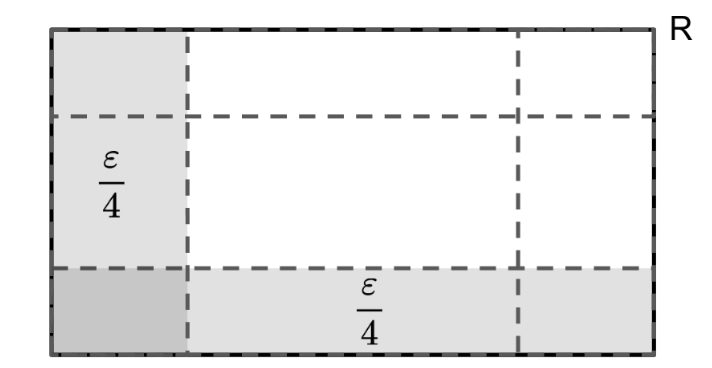
\includegraphics[width=0.4\textwidth]{assets/fig9.png}
    \caption{The 4 rectangles of area $\epsilon/4$}
    \label{fig:fig9}
\end{figure}

Let's consider the $m$ observations drawn from $p(\textbf{x}, y)$. If each of the four rectangles defined above contains at least one point, we have $error(h_m) \leq \epsilon$, because the area difference between $R$ and $R'$ would be fully covered by the 4 rectangles. 

\begin{figure}[H]
    \centering
    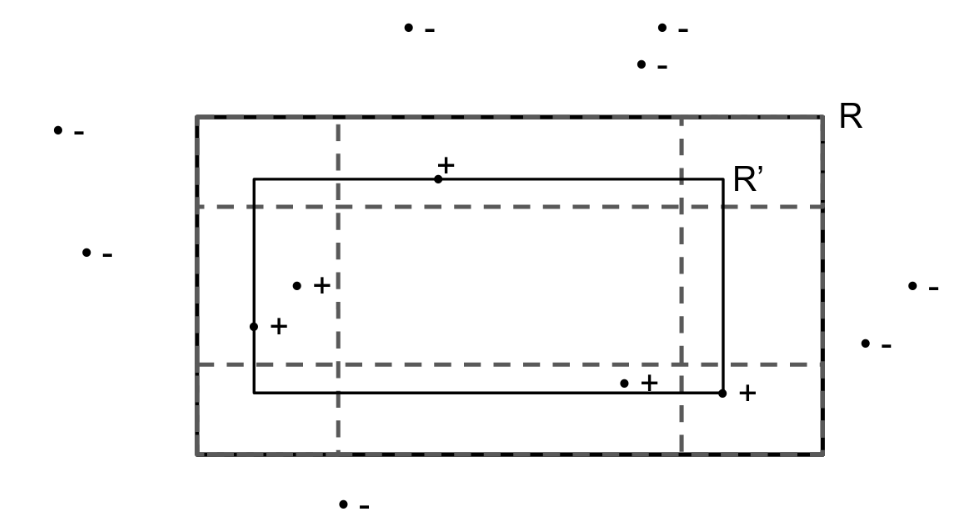
\includegraphics[width=0.4\textwidth]{assets/fig10.png}
    \caption{Configuration showing event}
    \label{fig:fig10}
\end{figure}

If we call this event $B$, we have: 
\[ 
    B \to error(h_m) \leq \epsilon 
\]

equivalently, by modus tollens:
\[ 
    error(h_m) > \epsilon \to \neg B
\]

This implies: 
\[ 
    P(\neg B) \geq P(error(h_m) > \epsilon)
\]

$P(\neg B)$ is the probability that at least one of the 4 rectangles doesn't contain any of the $m$ points. This probability is $(1-\epsilon/4)^m$ for a single rectangle, hence we have $P(\neg B) \leq 4(1-\epsilon/4)^m$. Thys the following chain of inequalities holds:
\[
    4(1-\epsilon/4)^m \geq P(\neg B) \geq P(error(h_m) > \epsilon)
\] 

Now, let $m_{\epsilon, \delta}$ be such that:
\[
    \delta \geq 4(1-\epsilon/4)^m_{\epsilon, \delta} \geq P(\neg B) \geq P(error(h_m) > \epsilon)
\]

Finding $m_{\epsilon, \delta}$ that satisfy this inequality would prove that $\forall m > m_{\epsilon, \delta}P(error(h_m) > \epsilon) \leq \delta$. We then require:
\[
    4(1-\epsilon/4)^m_{\epsilon, \delta} \leq \delta
\]

and we use the inequality $(1-k) \leq e^{-k}$ to obtain:
\[
    m_{\epsilon, \delta} \geq (4/\epsilon) \cdot \ln(4/\delta)
\]

In summary, provided a sample of at least $(4/\epsilon) \cdot \ln(4/\delta)$ examples in order to choose an hypothesis rectangle $R'$, we can assert that with probability at least $1- delta, R'$ will misclassify a new point (drawn according to the same distribution from which the sample was chosen) with probability at most $\epsilon$. 

This proves that our hypothesis set $\mathcal{H}$ is PAC-learnable.



\end{exampleblock}



\section{VC Dimension (Vapnik-Chervonenkis)}

Consider a class of hypotheses functions $\mathcal{H} = {h : X \to {0,1}}$ and a subset $C = {c_1,\dots, c_m} \subseteq X$ of input points. 

Define $\mathcal{H}_c = {(h(c_1),\dots, h(c_m))|h \in \mathcal{H}}$, the set of all tuples of Booleans obtained by applying all possible hypothesis functions $h \in \mathcal{H}$ to all points in C. We say that $\mathcal{H}$ \textbf{shatters} the set C iff |$\mathcal{H}_C| = 2^m$. 

Practically, this means that for any label assignment to points in C, we have a function in our hypothesis set which is able to match such an assignment. Namely, we can exactly describe every possible dataset with inputs in C. 

\begin{definitionblock}[VC Dimension]
    The \textbf{VC dimension of $\mathcal{H}$} is defined as:
    $$
    VC(\mathcal{H}) = \max \{m \in \mathbb{N} | \mathcal{H} \text{ shatters some } C \subseteq X, |C| = m\}
    $$
\end{definitionblock}

\textbf{Remark}: In calculating the VC dimension, it is enough that we find one set of m points that can be shattered, it is not necessary that we are able to shatter any m points. 

\begin{figure}[H]
    \centering
    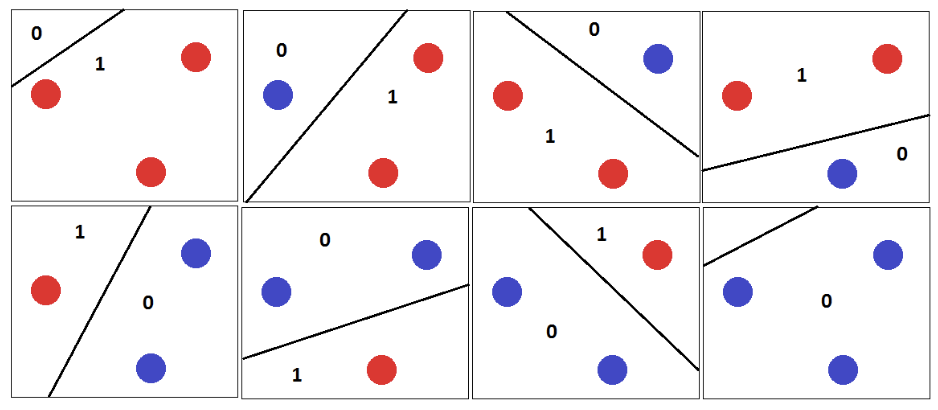
\includegraphics[width=0.7\textwidth]{assets/fig11.png}
    \caption{Proof that VCdim($\mathcal{H}_l \geq 3$)}
    \label{fig:fig11}
\end{figure}

\subsection{VC dimension and PAC learning}

In what follows, we will explore the reasons why VC dimension in crucial for PAC learnability. 


\begin{theorem}
    $If \mathcal{H} shatters C, |C| \geq 2m, then we cannot learn \mathcal{H} with m samples$
\end{theorem}

Hence, there will be an assignment of \textit{m} samples to classes in which we are going to commit a large error. 

\begin{figure}[H]
    \centering
    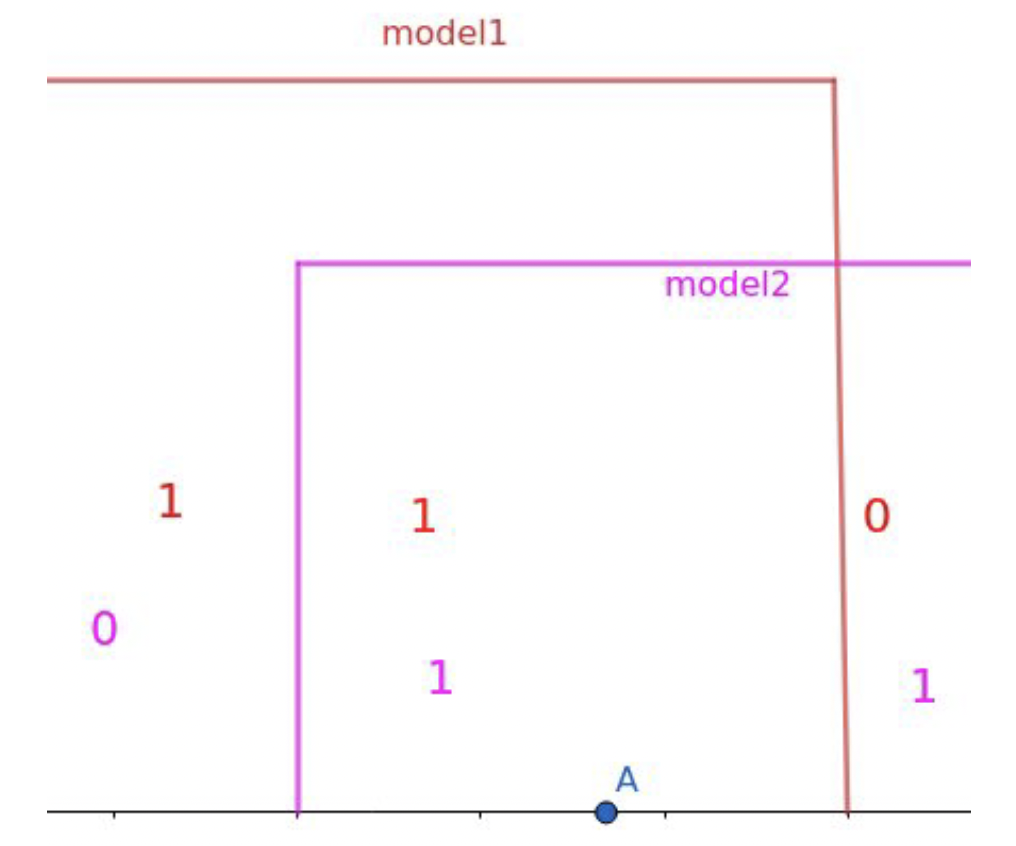
\includegraphics[width=0.2\textwidth]{assets/fig12.png}
    \caption{Visual interpretation of the theorem: it is impossible to train a model of type $\mathcal{H}_a+$ with only a point A with known classification, because the points different from A could have any classification.}
    \label{fig:fig12}
\end{figure}

If the $VCdim(\mathcal{H}) = \infty$, then $\mathcal{H}$ is not (agnostic) PAC learnable, indeed: 
\begin{theorem}
    $\mathcal{H} is (agnostic) PAC learnable iff VCdim(\mathcal{H}) < \infty$
\end{theorem}

In this case: $\exists c_1,c_2$ s.t.
$$
c_1 \frac{VCdim(\mathcal{H}) + \log (\frac{1}{\delta})}{\epsilon^2} \leq m_{\epsilon, \delta} \leq c_2 \frac{VCdim(\mathcal{H}) + \log(\frac{1}{\delta})}{\epsilon^2}
$$

Hence VC dimension gives us control on what we can or cannot learn. 

\subsection{Rademacher Complexity}

Consider the data generating distribution $p(x, y)$, a dataset $D ~ p^m$ and an hypothesis class $\mathcal{H} = {h : X \to {-1,1}}$.

\begin{definitionblock}[Rademacher Distribution]
    A distribution $\sigma = (\sigma_1, \dots, \sigma_m) s.t. \sigma_i \in {-1,1} \forall i and p(\sigma_i = 1) = 0.5$ is called \textbf{Rademacher Distribution}
\end{definitionblock}

\begin{definitionblock}[Rademacher Complexity]
    The \textbf{Rademacher Complexity} of $\mathcal{H}$ is defined as:
    $$
    R_m(\mathcal{H}) = \mathbb{E}_{\sigma} \left[ \sup_{h \in \mathcal{H}} \dfrac{1}{m} \sum_{i=1}^m \sigma_i h(x_i) \right]
    $$
\end{definitionblock}

\textbf{Remark}: this is a property both of the function \textit{h} and of the dataset \textit{D}.

\begin{observationblock}
$\sum_{i=1}^{m}\sigma_i h(x_i) = \sigma \cdot h(\underline{x})$ is the scalar product of the Rademacher distribution \sigma with the function \textit{h} evaluated on our dataset, so that $\frac{1}{m}\sigma \cdot h(\underline{x}) \in [-1,1]$, essentially is a measure of correlation of \textit{h} with random noise $\sigma$.
\end{observationblock}

Hence, for a specific choice of noise $\sigma$, we are going to look at the dataset and choose the best \textit{h} that correlates with this noise; then we take the expectation w.r.t. $\sigma$. 

\begin{definitionblock}[Rademacher Complexity]
    Taking into account the data generating mechanism \textit{p}, the \textbf{data-independent Rademacher complexity} is defined as:
    $$
    \mathcal{R}_m(\mathcal{H}) = \mathbb{E}_{D~p^m}[\hat{\mathcal{R}_D}(\mathcal{H})]
    $$
\end{definitionblock}

Fix $\mathcal{H} and p(x,y)$, then $\forall \sigma > 0$ with probability at least $1-\delta, \forall D ~ p^m, |D| = m, \forall h \in \mathcal{H}$ we have:
$$
\begin{array}{rl}
    R(h) \leq \hat(R_D)(h) + \underbrace{\mathcal{R}_m(\mathcal{H}) + \sqrt{\frac{\log (\frac{1}{\delta})}{2m}}}_{\epsilon_1}\\
    R(h) \leq \hat(R_D)(h) + \hat{\mathcal{R}_D}(\mathcal{H}) + 3\sqrt{\frac{\log (\frac{2}{\delta})}{sm}}_{\epsilon_2}
\end{array}
$$

\textbf{Remark}: computing the Rademacher complexity can be challenging, as it requires the solution of an optimization problem of any possible value of the Rademacher distribution. 

\subsection{Rademacher complexity and VC dimension}

\begin{definitionblock}[Growth Function]
    The \textbf{growth function} $\prod_{\mathcal{H}}$ is defined as:
    $$
    \prod_{\mathcal{H}} : \mathbb{N} \to \mathbb{N}, \prod_{\mathcal{H}}(m) = \max_{x_1,\dots,x_m \in X} |{\mathcal{H}_D}|, |D| = m
    $$
    with $\mathcal{H}_D = {h(x_1),\dots,h(x_m)|h \in \mathcal{H}, D = {x_1,\dots,x_m}}$
\end{definitionblock}

Hence the growth function describes how the complexity of what we can explain with out hypothesis set $\mathcal{H}$ increases with the cardinality of the data points that we have.

\begin{figure}
    \centering
    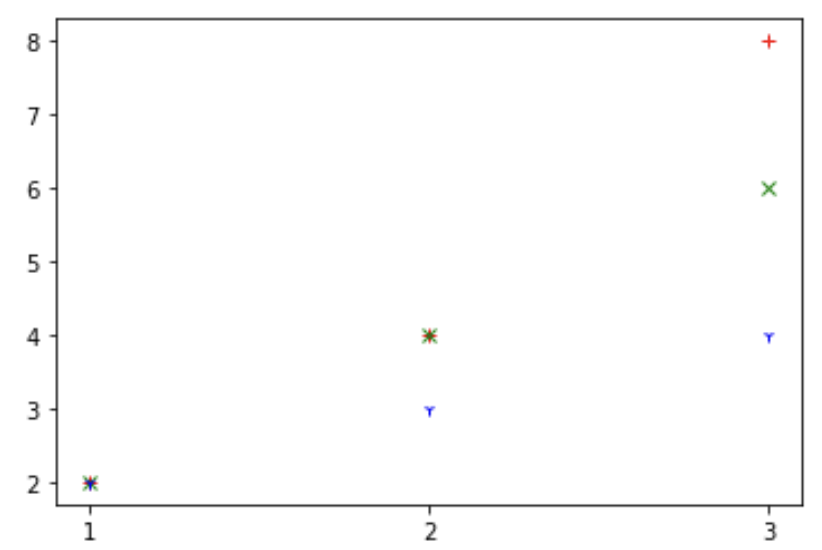
\includegraphics[width=0.7\textwidth]{assets/fig13.png}
    \caption{Plot of the growth functions of $\mathcal{H}_a$(blue), $\mathcal{H}_{a+}$(green), $\mathcal{H}_l$(red) for $1 \leq m \leq 3$}
    \label{fig:fig13}
\end{figure}

We can moreover define the $VCdim(\mathcal{H})$ in terms of the growth function:
$$
VCdim(\mathcal{H}) = \max \{m \in \mathbb{N} | \prod_{\mathcal{H}}(m) = 2^m\}
$$

Intuitively, this comes from the fact that if a set C is shattered by $\mathcal{H}$, then $\mathcal{H}_D = 2^m$.

\begin{theorem}[Sauer Lemma]
    $$
    \prod_{\mathcal{H}}(m) \leq \sum_{i=0}^{d} \binom{m}{i} \leq \left(\dfrac{em}{d}\right)^d \leq O(m^d)
    $$
    with $d = VCdim(\mathcal{H})$
\end{theorem}

Moreover it also holds that:
$$
\mathcal{R}_m(\mathcal{H}) \leq \sqrt{\dfrac{2\log(\frac{2}{\delta})}{m}} + \sqrt{\dfrac{2\log(\frac{2}{\delta})}{m}} \leq O(\sqrt{\dfrac{d}{m}})
$$

We can say that $\mathcal{R}_m(\mathcal{H})$ and $VCdim(\mathcal{H})$ are essentially equivalent, in the sense that when the VC dimension is $\infty$ then the upper bound on the Redemarcher complexity is independent of \textit{m} and greater than 1 (if you substitute it into the PAC bound using Redemacher complexity, you get an error which remains always large, no matter how large is \textit{m}). Otherwise, when the VC dimension is $< \infty$, the bound tends to go to 0 as \textit{m} grows to infinity. 

Summarizing, we have ways to measure the complexity of our hypotheses
space: if this complexity is finite (in the sense of VC dimensionality), then
what we have as a result is that we can constrain the error and provide
bounds that tell us that this error is going towards 0, as we increase the
data points (i.e. we will eventually learn). Instead if the VC dimension is
infinite, no matter how many data points we have, we are not going to be
able to learn, because the complexity of our model is too high, hence it
can always overfit the data.

Hence, in order to be able to actually learn, we need to put some
constraints in our hypothesis set, and this formalizes our inductive
bias.
